% This is an LPSC Abstract template for LaTeX 2e that is based off of the
% LaTeX article document class.

% $Id$

% Copyright (C) 2005,2007 Ross A. Beyer
% Copyright (C) 2008 Ross A. Beyer and Moses P. Milazzo

% This work is licensed under the Creative Commons
% Attribution-Noncommercial-Share Alike 3.0 License. To view a copy
% of this license, visit http://creativecommons.org/licenses/by-nc-sa/3.0/;
% or, (b) send a letter to Creative Commons, 171 2nd Street, Suite
% 300, San Francisco, California, 94105, USA.

% Use the LaTeX article class.  Pass any options you like to article, except
% twocolumn.  We take care of that in the lpscabs pacakage below.
\documentclass[twoside]{article} 

\usepackage{times}				% Nice fonts, optional
\usepackage{url}                % Needed for wrapping long URLs

\usepackage{graphicx}			% Nice graphics, optional

\usepackage[numbers]{natbib}	% Nice references, optional
% These next three commands are relevant to natbib.  If you don't use
% natbib for your references, you should get rid of these, as well.
\newcommand{\bibfont}{\small}	% Change the font size of the bibliography
\setlength{\bibsep}{0pt}		% Remove the spacing between bib entries
\renewcommand{\bibsection}{\subsubsection*{\refname}}
								% Make the References heading smaller.

% To compress the section titles even more, use the titlesec package.
%\usepackage[small,compact]{titlesec}

% \usepackage{paralist}			% For compressing bibliography into a paragraph

% \usepackage{balance}			% For balancing columns on the page.
								

\usepackage{lpscabs}			% This is to take care of some LPSC abstract
								% document-specific things and set sizes.

\usepackage[pdftex,colorlinks=true,urlcolor=blue,citecolor=black,linkcolor=black]{hyperref}
								% Puts actual hyperlinks in your PDF, optional.

\begin{document}

% The \titlearea command takes two arguments in curly braces {}.  The first
% will be used as the title, and the second as the author info.

\titlearea{Using \LaTeX\ to write an LPSC Abstract.}{Ross A. Beyer$^{1,2}$ and Moses P. Milazzo$^{3}$, $^1$Carl Sagan Center at the SETI Institute, $^2$NASA Ames Research Center, MS 245-3, Moffett Field, CA, USA (\href{mailto:Ross.A.Beyer@nasa.gov}{Ross.A.Beyer@nasa.gov}), and $^3$Astrogeology Branch, United States Geological Survey}

% Here is an example with just one author:
%
%\titlearea{Using \LaTeX\ to write an LPSC Abstract.}{Ross A. Beyer, NASA Ames Research Center, MS 245-3, Moffett Field, CA, USA (Ross.A.Beyer@nasa.gov)}

% Here is an example with more than one author from more than one place:
%
% \titlearea{Using \LaTeX\ to write an LPSC Abstract.}{Ross A. Beyer$^{1,2}$, John Q. Public$^{a}$, and Jane Doe$^{\dag}$, $^1$Carl Sagan Center at the SETI Institute, $^2$NASA Ames Research Center, MS 245-3, Moffett Field, CA, USA (Ross.A.Beyer@nasa.gov), $^{a}$123 Sesame Street, New York NY, USA, $^{\dag}$890 Somewhere, ID, USA}

% The LPI no longer recommends using a running title.
% % If your abstract is two pages long, type your running head in the argument
% % below:
% \runningtitle{\LaTeX\ and the LPSC Abstract, R. A. Beyer and M. P. Milazzo}

% Uncomment \usepackage{balance} above to use this:
% \balance

There used to be a \LaTeX\ template and a style file for writing
Lunar and Planetary Science Conference (LPSC) abstracts available
on the LPSC Web site.  However, in the last couple of years, no
such template has been available, and we found ourselves dragging
the old one out.  It was full of scary \TeX\ commands and had a
date from 1996 in it, so we decided to start from scratch and write
a \href{http://rossbeyer.net/software/lpsc_template/}{template} based 
on \LaTeX's own article class and a short \LaTeXe\
package file.  Most of the \LaTeX\ work is based on \citet{latexguide}.

Fortunately, the requirements for LPI-sponsored meeting abstracts (like LPSC)
are reasonably relaxed.

\subsubsection*{Title area}

The title mechanism for this template is a simple command,
\verb=\titlearea=, which takes two arguments, the title text and the
author info text.

The title text is made a font size bigger and made boldface in the
lpscabs package.  If you would like it styled differently, it should
be easy to go in to the \texttt{lpscabs.sty} file and change it.

The old style file had a fancy automatic mechanism for entering
authors and putting superscripted numbers on their names to match
up with their affiliations later on in the title.  We contemplated
doing that and then realized that maybe authors would like some
other mechanism besides numbers, maybe little letters, or any of
the special characters like \dag\ or \ddag\ to mark their affiliations,
or maybe all of the authors are from the same place, so no little
super-scripted characters are needed.  Possibly some authors could
have more than one affiliation.  So rather than try to program
something that can be all things to all people, we'll just let you
(the authors) do whatever you like to the text in that line, you're
smart people.  It is a little less convenient, but we think it is more
flexible.  We have commented out a few multiple author styles up
near that section of this source file.

% The LPI no longer recommends using a running title, since they 
% actually add a header to both pages of the PDF these days.
% \subsubsection*{Running title}
% 
% If your abstract is two pages, and you'd like to have a snappy little
% header on the second page, then you can use the \verb=\runningtitle=
% command to supply text that will be written there.

\subsubsection*{Section styles}

In general, people try to put lots of information into their LPSC
abstracts, and want to minimize the space being taken up by section
headers.  You could redefine the sectioning commands to change their
styling if you like, or you could just use the \verb=\subsubsection*=
command (as we have done in this example), and
you could even use the \verb=\paragraph= command if you wanted the
section's title on the same line as the first sentence of the
section, saving even more space.  You can also use the \texttt{titlesec}
package with the \texttt{small} and \texttt{compact} options to further
compress the font size and space around titles.


\subsubsection*{Figures}

\begin{figure}
\begin{center}
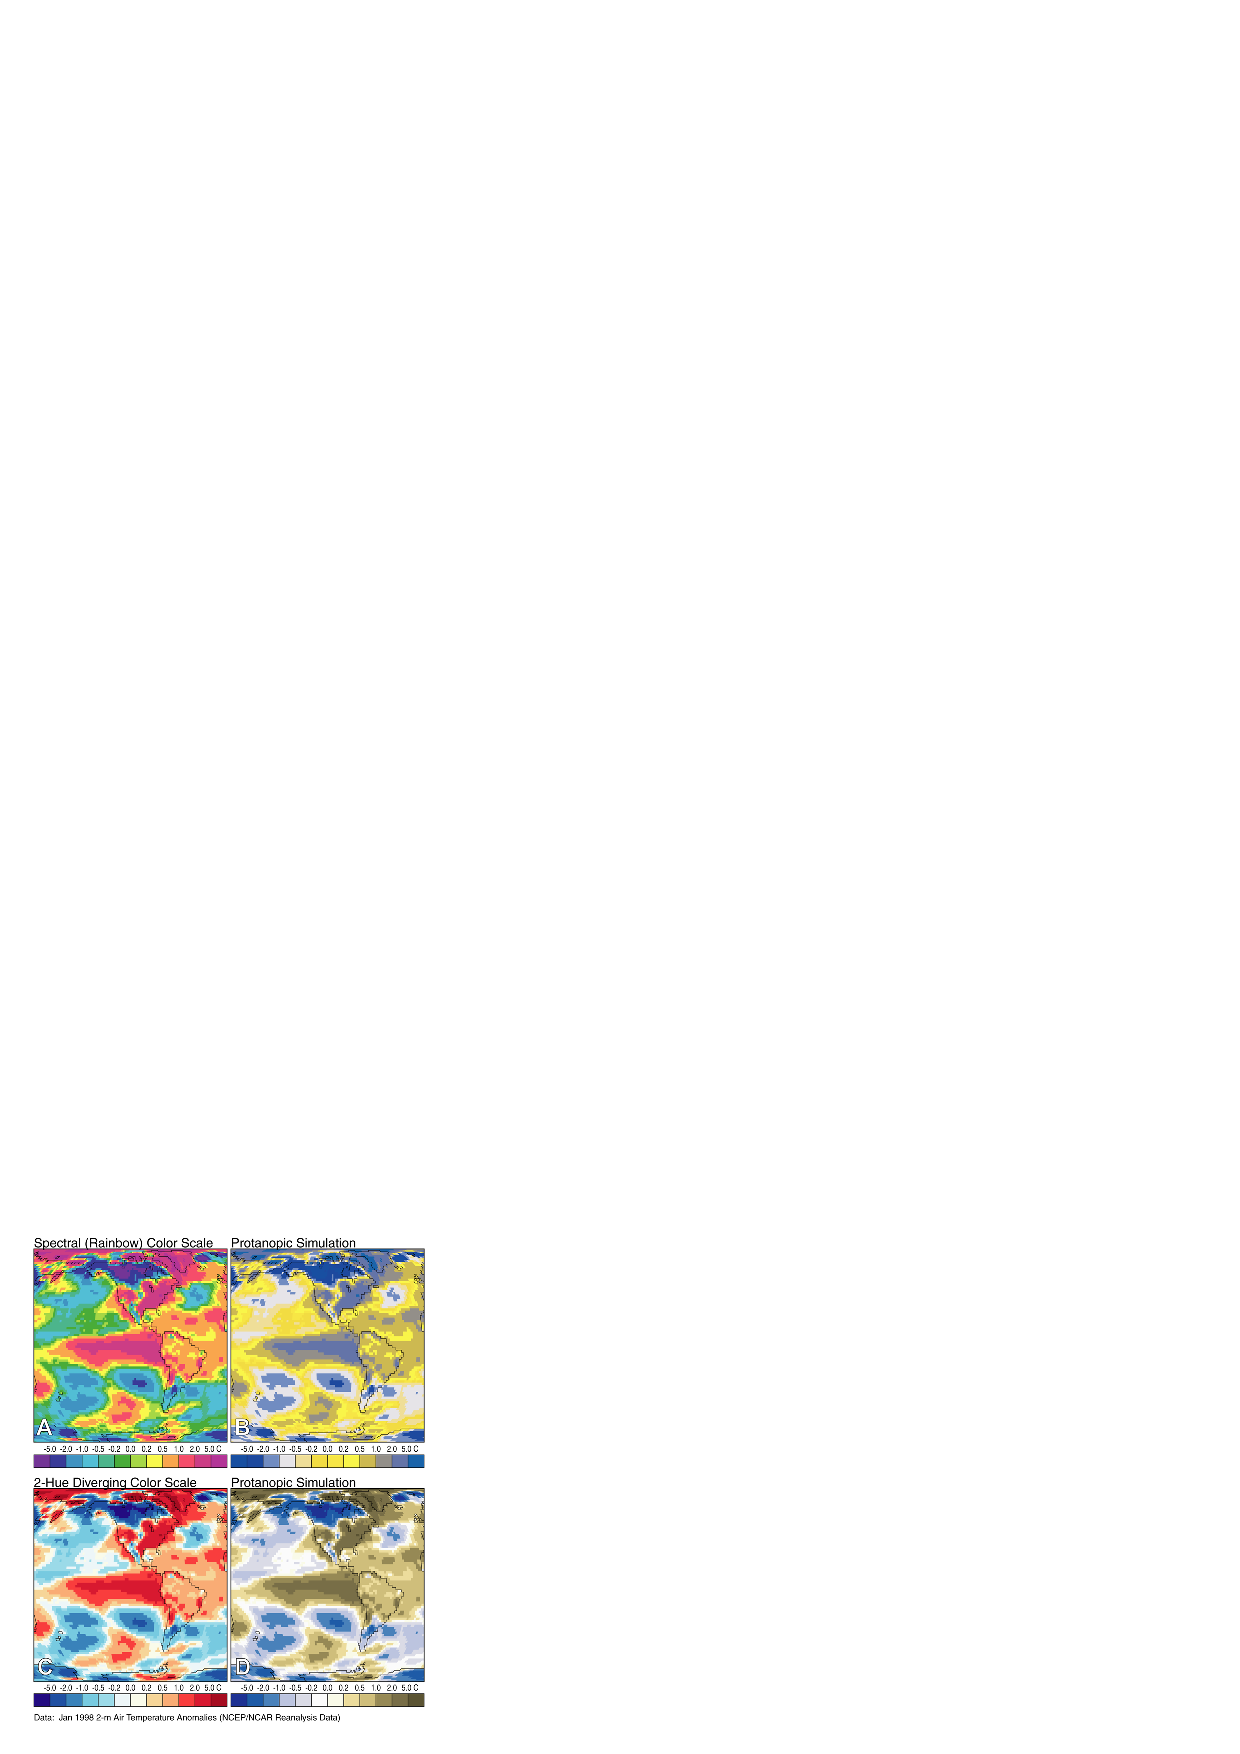
\includegraphics[width=\columnwidth]{lb_fig1.png}
\caption[Color Scales and Color-Deficient-Viewer Simulations]{
    \label{color_scales}
    This is Figure 1 from \citet{2004EOSTr..85..385L}.  
    }
\end{center}
\end{figure}

Good figures are hard to make, there's no question about it.  That
goes double for deciding which figures to include in your 
space-limited abstract.

When you make the decision to create a color figure, take some time
to think about the colors that you use.  We think that
\citet{2004EOSTr..85..385L} make a good case for not using the
typical rainbow-spectrum color scheme (e.g. Fig.~\ref{color_scales}).
Just because you decide to use color doesn't mean that you need to
use \emph{all} of the colors.  Don't confuse ``pretty'' with
``meaningful.''

If you need figures or tables to be the full width of the page,
just use their starred versions, like \verb=\begin{figure*}= instead
of \verb=\begin{figure}=.

\subsubsection*{URLs and hyperlinks}

Let's face it, the odds are good that more people will read this
abstract on their computer screens via a PDF reader than will do
so on paper.  Fortunately, PDFs can contain active hyperlinks that
can fire off a Web browser, or your e-mail client, and the
\verb=hyperref= package helps you do this.  It is used in this
example file, and there are blue links that you can click on in
this document, try them out.

The \verb=hyperref= package has some options that we should probably 
detail.  Here's a copy of the command in this document (carriage returns 
included for clarity):

\begin{verbatim}
\usepackage[pdftex,colorlinks=true,
  urlcolor=blue,citecolor=black,
  linkcolor=black]{hyperref}
\end{verbatim}
\noindent
The options in the square brackets are important, and
\url{http://www.tug.org/applications/hyperref/manual.html} details
all of them.  The first item \verb=pdftex= is because we mostly use
\verb=pdflatex= to create PDF files from our \verb=.tex= files.  If
you use \verb=ps2pdf=, or something else, you'll want to specify
something else here.  The \verb=colorlinks= and \verb=urlcolor=
options should be reasonably self-explanatory, but you may wonder
why we set \verb=citecolor= and \verb=linkcolor= to black.  The
\verb=hyperref= package is good, it actually creates links for all
kinds of things in the document, and gives them unique link colors.
However, in this short document, that's kind of overkill, and a
little visually distracting.  So the links are still there, its
just that the text is black.  So go ahead and click on the references
numbers, like this one: \citep{latexguide} (which won't do much since
the references are on this page), or figure numbers like
this: \ref{color_scales}, and you'll get hopped to the right page.


\subsubsection*{Copyright Information}

This work is licensed under the Creative Commons
Attribution-Noncommercial-Share Alike 3.0 License. To view a copy
of this license, visit \url{http://creativecommons.org/licenses/by-nc-sa/3.0/};
or, (b) send a letter to Creative Commons, 171 2nd Street, Suite
300, San Francisco, California, 94105, USA.

Does this mean that if you write an abstract using this template that
you are required by law to credit us and to release the paper under
the same kind of Creative Commons license?  No, it doesn't.  Mostly
for the same reasons that you don't credit the authors of \LaTeX\
when using their software to create documents.  What it does do is allow
anyone, even the LPI Meeting Staff, to take a copy of this template
and modify it (or not), and place it on their web pages for folks
to use.

Why not just dedicate it to the public domain, you might ask?  Well,
we did spend some time on it and would like to be recognized.  Using
the Creative Commons license above allows us to retain copyright,
request that derivative templates credit us, but also allow for
\emph{anyone} to make derivative works, in addition to a few other
rights and restrictions.  If you want to know more, visit the
Creative Commons web site.  You may even want to check out the
Science Commons at \url{http://sciencecommons.org/}.


\subsubsection*{Works that you reference}

Using \texttt{natbib} with the \texttt{numbers} option and the
\texttt{unsrtnat} bibliographystyle approximates the reference-style
that has emerged for LPSC abstracts over the years, but there is
no hard and fast rule.  You may think that the references take up
too much vertical space (with each reference starting a new line).
You can use the \texttt{paralist} package and enclose the bibliography
stuff in a \texttt{inparaenum} environment (which is itself enclosed
in a \texttt{flushleft} environment).  Examples of how to do this
are commented out in this source file.  Of course, you don't have to 
use \texttt{natbib}, if you don't want to.  However, if you really have
that many references maybe you should be submitting this to a
peer-reviewed journal and not just a conference.

% Uncomment \usepackage{paralist} above to use the inparaenum environment.
% \begin{flushleft}
% \begin{inparaenum}
\bibliography{bibliography}
\bibliographystyle{unsrtnat}
% \end{inparaenum}
% \end{flushleft}

\end{document}

